\documentclass[a4paper,fleqn]{cas-sc}

\usepackage[authoryear]{natbib}
\usepackage{amsmath,amssymb,booktabs,tabularx,graphicx,capt-of}
\usepackage{url}
\usepackage{acro}

% Target journal: Engineering Applications of Artificial Intelligence.
\newcommand{\targetjournal}{Engineering Applications of Artificial Intelligence}

\ExplSyntaxOn
\cs_set:Npn \__first_footerline:
{
  \group_begin:
  \small
  \sffamily
  \ifnum\theblind>0\relax
  \else
    \__short_authors: :~
  \fi
  { \rmfamily \itshape Preprint~ submitted~ to~ \targetjournal }
  \group_end:
}
\ExplSyntaxOff

\DeclareAcronym{ai}{short=AI,long=Artificial Intelligence}
\DeclareAcronym{vv}{short=V\&V,long=Verification and Validation}
\DeclareAcronym{mis}{short=MIS,long=Mechanistic Identifiability Score}
\DeclareAcronym{vbn}{short=VBN,long=Visual Behavior Neuropixels}
\DeclareAcronym{ccf}{short=CCF,long=Common Coordinate Framework}
\DeclareAcronym{v1}{short=V1,long=primary visual cortex}
\DeclareAcronym{bmtk}{short=BMTK,long=Brain Modeling ToolKit}
\DeclareAcronym{tvb}{short=TVB,long=The Virtual Brain}
\DeclareAcronym{microns}{short=MICRONS,long=Machine Intelligence from Cortical Networks}
\DeclareAcronym{cave}{short=CAVE,long=Connectome Annotation Versioning Engine}
\DeclareAcronym{svd}{short=SVD,long=singular-value decomposition}
\DeclareAcronym{mlp}{short=MLP,long=multilayer perceptron}
\DeclareAcronym{bold}{short=BOLD,long=blood-oxygen-level-dependent}

\begin{document}
\let\WriteBookmarks\relax
\def\floatpagepagefraction{1}
\def\textpagefraction{.001}


\shorttitle{Claim-aware validation of mouse-brain models}
\shortauthors{Anonymous}

\title[mode=title]{MouseBrainBench: A claim-aware validation framework for partial
mouse-brain digital models}


\author[1]{Anonymous Author}
\affiliation[1]{organization={Affiliation withheld for double-anonymized review},
                country={}}


\begin{abstract}
Artificial Intelligence (AI)-based computational models are increasingly used to support engineering decisions in complex scientific domains, but their evaluation often relies on predictive performance while reported interpretations concern reproducibility, anatomical fidelity, or mechanism. This paper presents MouseBrainBench, a claim-aware verification and validation framework for partial mouse-brain digital models. The AI contribution is an executable, non-compensatory audit process that separates prediction, reproducibility, topology specificity, directed identifiability, local structure--function agreement, and computational cost through a Mechanistic Identifiability Score and a conjunctive claim gate. The engineering application is the validation of neurocomputational digital model targets built from public mouse-brain resources. MouseBrainBench is evaluated with controlled simulations, Allen Visual Behavior Neuropixels, Static and Dynamic Sensorium, and Machine Intelligence from Cortical Networks (MICrONS). Synthetic cases recover the intended decision semantics, while Allen and Sensorium act as negative or bounded predictive cases that are not promoted to mechanism. The main positive empirical case is a local MICrONS structure--function analysis: across one discovery cohort and two non-overlapping hold-out windows from the same resource, connected directed pairs show greater readout-location similarity than distance- and degree-matched controls. These results support an internally reproduced local association, not a causal, behavioural, or whole-brain digital twin. MouseBrainBench therefore provides a reproducible engineering framework for deciding which claims about AI-based scientific models are supported, partially supported, or not supported by the available evidence.
\end{abstract}


\begin{keywords}
Artificial Intelligence Validation \sep Scientific Machine Learning \sep
Digital Twins \sep Computational Neuroscience \sep Benchmarking \sep
Mechanistic Identifiability
\end{keywords}


\maketitle
\acresetall


\section{Introduction}
\label{sec:introduction}

Computational representations of biological systems have become a key point in
the interaction between \ac{ai} and neuroscience. In the case of the laboratory
mouse (\textit{Mus musculus}), several public infrastructures provide standardised
neurophysiological recordings, visual-response benchmarks, anatomical atlases,
and electron-microscopy reconstructions. These resources allow researchers to
analyse the same biological system from different perspectives, ranging from
population activity recorded across brain regions to synaptic connectivity in a
restricted cortical volume. Therefore, they also facilitate the development of
models that reproduce selected observations with increasing accuracy.

However, this progress also generates a relevant validation problem. A model
that predicts neural responses is not necessarily a model that identifies the
circuit producing them. A response can be stable across animals while remaining
compatible with several alternative topologies. Similarly, a model can preserve
an anatomical graph without demonstrating that its directed dynamics are
identified by the available observations. Notice that predictive performance,
empirical reliability, anatomical plausibility, and causal explanation answer
different scientific questions. Thus, a single correlation coefficient is not
sufficient to decide whether a model supports a mechanistic claim.

This distinction is especially important when digital-twin terminology is used.
A digital twin normally implies correspondence with a specific physical entity,
repeated calibration, and the ability to reproduce relevant states under
meaningful interventions. Current mouse-brain resources do not jointly provide
complete synaptic connectivity, full-brain dynamics, behaviour, and
interventional validation for an individual animal. \ac{microns} offers
exceptional synaptic and functional detail, but only for a local visual-cortical
volume \citep{bae2025microns}. Allen datasets provide broad and standardised
neural recordings, but not the individual synaptic graph that generated each
response \citep{siegle2021survey}. Consequently,
treating either resource as a complete mouse-brain twin would exceed the
available evidence.

Existing software and benchmark infrastructures already solve relevant parts of
this problem. \ac{bmtk} provides tools for constructing and simulating multiscale
neural networks \citep{dai2020bmtk}. \ac{tvb} supports connectome-based
population dynamics \citep{tvb2013}. Sensorium provides common predictive tasks
for mouse visual cortex \citep{willeke2022sensorium,turishcheva2023dynamic}.
For this reason, the main gap is not the absence of another simulator or another
visual-response leaderboard. The unresolved point is the audit between a metric
and the biological claim attached to it: what evidence is required before a
reproducible prediction can be interpreted as support for a specific mechanism?

In accordance with this objective, this paper presents MouseBrainBench, a
claim-aware validation framework for partial mouse-brain digital models. It is
not proposed as a complete brain simulator and it does not claim to instantiate
a full digital twin. The framework assigns public datasets to explicit
evidential roles, evaluates them using matched null models and hold-out checks,
and records which interpretations are admitted or blocked. Its Mechanistic
Identifiability Score (MIS) is not a conventional weighted ranking. It is a
conjunctive decision procedure over non-interchangeable evidence blocks.

From the perspective of Engineering Applications of Artificial Intelligence, MouseBrainBench is framed as an AI engineering contribution rather than as a new biological simulator. The AI contribution is the executable claim gate: a non-compensatory validation layer that turns qualitative model claims into auditable decisions. The engineering application is the validation of partial neurocomputational digital models before they are used to support scientific or technical interpretation. This formulation also provides a measurable advantage over conventional predictive evaluation, because it identifies cases in which a high predictive or reproducibility score would incorrectly promote an unsupported mechanistic claim.

The proposal is evaluated through positive and negative cases. Four synthetic
systems are used to test whether the MIS recovers known truth and rejects
common-drive or incomplete mechanisms. Allen Visual Behavior Neuropixels is used
to verify that the framework can keep a highly reproducible empirical target
while rejecting unsupported topology and direction claims. Static and Dynamic
Sensorium are used to preserve predictive evidence without promoting it to
causality. Finally, MICRONS is used to test a discovery-fixed local
structure--function endpoint against distance- and degree-matched nulls in a
discovery cohort and two non-overlapping hold-outs. This sequence evaluates the
audit procedure itself, not a collection of unrelated dataset demonstrations.

The rest of the article is organised as follows. Section~\ref{sec:contributions}
details the research contributions of the proposal. Section~\ref{sec:related-work}
reviews the most relevant predictive, simulation, and connectomic approaches.
Section~\ref{sec:framework} describes the MouseBrainBench framework and its
main components. Section~\ref{sec:evaluation} presents the experimental
evaluation and the achieved results. Section~\ref{sec:discussion} discusses the
scope and limitations of the proposal. Finally, Section~\ref{sec:conclusions}
concludes the paper and provides future guidelines.

\section{Research contributions}
\label{sec:contributions}

The main innovation of MouseBrainBench lies in its explicit separation between
model performance and the scientific claim derived from that performance. The
framework does not try to replace existing simulators or predictive benchmarks.
Instead, it provides a reproducible mechanism to decide whether a partial digital
model supports a predictive, reproducibility, structure--function, or
mechanistic-identifiability claim.

The contributions of the proposal are summarised in the following points:

\begin{itemize}
  \item The proposal introduces a claim-aware validation formulation that
  separates prediction, reproducibility, topology specificity, directed
  identifiability, local structure--function association, and computational
  cost. This fact allows the system to return not only a numerical result, but
  also an explicit set of admitted and rejected interpretations.

  \item A formal \acs{mis} is defined through non-interchangeable evidence
  blocks and fixed directional thresholds. The rule is evaluated with four
  known-truth systems that isolate common drive, topology without direction, and
  direction without topology specificity. These experiments validate the
  operational semantics of the claim gate, rather than providing an exhaustive
  Monte Carlo characterization of false-positive or false-negative rates.

  \item A cross-resource protocol is established by assigning Allen,
  Sensorium, Dynamic Sensorium, and \acs{microns} different roles in the
  validation process. Thus, heterogeneous datasets are not mixed as if they were
  repeated measurements of the same system. Allen acts as a real negative
  mechanistic control, Sensorium as a predictive control, and \acs{microns} as a
  local anatomical-functional case.

  \item A MICRONS validation case is provided using a discovery-fixed primary
  endpoint, distance- and degree-matched null models, false-discovery-rate
  correction, unit-cluster bootstrap stability intervals, and two non-overlapping hold-out
  windows. The aim is to recover a bounded and previously motivated local
  structure--function phenomenon, not to claim a new general wiring rule.

  \item The work includes a reproducible publication freeze that links numerical
  artifacts with allowed and blocked claims. In the current study, the framework
  admits an internally reproduced local observational structure--function association, while
  rejecting causal, behavioural, whole-brain, and state-of-the-art predictor
  claims. This produces a direct advantage over a conventional predictive
  evaluation, because strong reproducibility or prediction in Allen and Sensorium
  is not allowed to compensate for missing topology, direction, or causal
  evidence.
\end{itemize}

Notice that these contributions define the scope of the paper. MouseBrainBench
is a framework for evaluating the relationship between evidence and
interpretation. It does not establish that a single score is universally
sufficient for mechanistic neuroscience. The MIS thresholds and evidence blocks
must be specified according to the target claim before evaluation, and a failure
means that the analysed claim is not supported, not that the dataset or model is
without scientific interest.

\section{Related work}
\label{sec:related-work}

This section introduces the foundations on which MouseBrainBench is based. The
proposal is related to neural-response prediction, multiscale brain simulation,
connectomics, and model-credibility research. These areas share data sources and
biological targets, but they do not validate the same kind of scientific claim.
For this reason, the literature is revisited according to the evidence that each
approach can provide.

First, model credibility and claim documentation are considered, because they
provide the conceptual basis for separating intended use, validation evidence,
and final interpretation. Second, standardised recordings and predictive
benchmarks are reviewed, with special attention to the limits of response
prediction. Third, multiscale simulation and digital-brain models are discussed,
including tools that already provide mature simulation infrastructures. Finally,
connectomic and structure--function studies are addressed, as they are the basis
for the MICRONS validation case.

\subsection{Model credibility and claim documentation}
\label{subsec:model-credibility}

The central problem is a model-credibility problem rather than only a neural
modelling problem. Verification and validation frameworks distinguish whether a
model is implemented correctly, whether it is adequate for a specified intended
use, and how uncertainty affects that intended use
\citep{asme2018vv40,oberkampf2010verification,sargent2013verification,riedmaier2021vvuq}.
This literature is important for MouseBrainBench because it treats credibility as
conditional on a declared decision, not as a property that follows automatically
from a high global score. A model can therefore be credible for prediction and
not credible for a causal or mechanistic claim.

Machine-learning reporting practices make a similar point from the opposite
side. Datasheets, model cards, and reproducibility checklists document intended
uses, evaluation data, limitations, and execution conditions
\citep{gebru2021datasheets,mitchell2019modelcards,pineau2021reproducibility}.
MouseBrainBench imports this discipline into computational neuroscience by
binding every result to a claim contract, a set of controls, and a publication
freeze. The freeze is not merely archival: it prevents post-hoc expansion of the
claim after inspecting additional endpoints.

Digital-twin reviews also caution against equating any executable simulation
with a twin. Mature digital-twin definitions emphasize linkage to a physical
entity, lifecycle data exchange, uncertainty, and intended use
\citep{jones2020digitaltwin,rasheed2020digitaltwin,fuller2020digitaltwin,shao2022credibility}.
This supports the restricted terminology used here: MouseBrainBench audits
partial digital representations, while complete mouse-brain twin claims remain
blocked unless entity-specific calibration, broad state coverage, and
intervention-level validation are available.


\subsection{Standardized neural recordings and response prediction}
\label{subsec:recordings-prediction}

The Allen Brain Observatory has made standardized neurophysiological data from
the mouse visual system available at a scale that supports comparisons across
sessions, animals, and analysis pipelines \citep{siegle2021survey}. The Visual
\ac{vbn} resource is especially relevant because it combines
large-scale extracellular recordings with controlled visual and behavioural
conditions. Standardization and public access improve reproducibility, but the
recordings remain observations of activity. They do not provide the complete
synaptic graph of each recorded animal, and several latent circuits can generate
similar population responses.

Cross-resource integration also depends on anatomical standardization. The Allen
Mouse Brain \ac{ccf} provides a three-dimensional reference
atlas derived from 1675 brains at 10-$\mu$m voxel resolution
\citep{wang2020ccf}. This makes regional alignment and aggregation possible,
but a reference atlas is not an individual connectome. MouseBrainBench therefore
uses atlas identity as provenance and anatomical context rather than as evidence
that subject-specific wiring has been observed.

Whole-brain axonal tracing supplies a complementary mesoscale view. The Allen
Mouse Brain Connectivity Atlas established a brain-wide projection map
\citep{oh2014mesoscale}, and subsequent modelling inferred connectivity at
100-$\mu$m voxel resolution under spatial smoothness assumptions
\citep{knox2019connectome}. These resources are indispensable for regional and
voxel-scale models, but inferred projection strength is not a measured
single-neuron connectome. The distinction between measured and inferred
structure is therefore part of the provenance recorded by MouseBrainBench.

Sensorium introduced a complementary evaluation regime: predicting large-scale
neural responses to static natural images in mouse primary visual cortex
\citep{willeke2022sensorium}. Dynamic Sensorium extended the task to videos,
behavioural covariates, and out-of-distribution evaluation
\citep{turishcheva2023dynamic,turishcheva2024retrospective}. These competitions
have advanced model architectures, shared evaluation, and reproducible data
handling. Correlation with held-out neural responses is a meaningful measure of
functional approximation and can identify models that generalize better than
simple baselines.

Neural-response metrics must account for response variability and the
reliability ceiling of the recorded neurons \citep{schoppe2016performance}.
Recent foundation models extend prediction to new visual stimulus types and
provide functional descriptors for the MICRONS animal
\citep{wang2025foundation}. These advances strengthen predictive models as
experimental tools, while making it more important to state whether a reported
value measures raw prediction, reliability-normalized performance, or evidence
about circuit organization.

The term \emph{digital twin} is also used for neural response models that enable
experiments in stimulus space. Recent work on visual-cortex digital twins shows
that functional surrogates can be scientifically useful while still requiring
careful population-level validation. In particular, Liscai et al. found that
models can match single-neuron responses while failing to reproduce relevant
properties of
population-response geometry \citep{liscai2025population}. Their result provides
a direct example of metric-dependent validation. It supports the need to match
the evaluation target to the intended use and to avoid treating one predictive
score as evidence for every level of neural organization.

Nevertheless, predictive equivalence does not imply mechanistic equivalence.
Two architectures can generate similar held-out predictions while relying on
different internal representations. High response correlation therefore
supports a predictive-surrogate claim, conditional on reliability and test
design, but not by itself an anatomical or causal claim. MouseBrainBench retains
the established predictive metrics and adds an explicit boundary: predictive
results enter the audit as one evidence type and cannot satisfy absent topology
or directionality requirements.

\subsection{Multiscale simulation and digital-brain models}
\label{subsec:multiscale-simulation}

Biologically grounded simulators address a different problem. \ac{bmtk}
provides interfaces and workflows for constructing networks from cellular and
connectivity information and executing them at different levels of resolution
\citep{dai2020bmtk}. SONATA-compatible descriptions improve
portability between tools. At a coarser scale, \ac{tvb} models
population dynamics over connectomes and supports the study of large-scale
network behaviour \citep{tvb2013}. These systems demonstrate that simulation
engines, model formats, and numerical integration are already mature research
infrastructures.

Mouse-specific models further reduce the space in which a new simulator would
be novel. The Virtual Mouse Brain extends connectome-based population dynamics
to tracer- and imaging-derived mouse connectomes
\citep{melozzi2017virtualmouse}. At circuit scale, the Allen V1 model integrates
cellular, structural, and functional measurements into biophysically detailed
and point-neuron networks \citep{billeh2020v1}. MouseBrainBench does not compete
with either contribution. It evaluates whether outputs from such models support
the claim attached to them.

Digital Twin Brain proposals broaden this objective towards multiscale models
that connect biological and \acs{ai} \citep{xiong2023dtb}. These proposals are
relevant to the present work because they move beyond isolated response
prediction and consider how anatomical, functional, and computational evidence
can be combined. However, a multiscale architecture does not by itself determine
which claim has been validated. Inferred single-neuron connectivity does not
become an observed individual connectome solely because a model matches a
macroscopic signal. Likewise, high \acs{bold} correlation does not establish that
the inferred wiring is uniquely identified. MouseBrainBench therefore treats
such systems as candidates for audit rather than as direct competitors.

This landscape changes the novelty criterion for the present work. Rebuilding a
spiking engine or a connectome-based neural-mass simulator would duplicate
established technology without resolving whether the resulting output justifies
a biological claim. Conversely, successful numerical execution only establishes
that a model is computationally well posed under its assumptions. Biological
validity still depends on parameter provenance, target observability, null-model
comparisons, and evaluation under perturbations or independent data.

MouseBrainBench is therefore positioned above, rather than instead of, these
tools. An external simulator may produce candidate dynamics. The benchmark
records the target, controls, and evidence required to interpret them. This
separation also prevents the phrase \emph{digital twin} from being used as a
synonym for any executable brain model. The present framework reserves stronger
twin claims for systems that can demonstrate entity-specific calibration,
state-dependent prediction, and suitable interventional validation.

\subsection{Connectomics and structure--function analysis}
\label{subsec:connectomics}

Electron-microscopy connectomics offers the most direct local evidence about
synaptic wiring. \acs{microns} links a dense reconstruction of mouse visual cortex to
functional measurements and related cell properties \citep{bae2025microns}.
It is therefore suitable for asking whether connected neurons share functional
properties more strongly than comparable non-connected neurons. Unlike a
response-only dataset, \acs{microns} permits connectivity and functional descriptors
to be tested within a co-registered local population.

The combination of in vivo functional characterization and electron microscopy
predates \acs{microns}. Earlier work demonstrated that network anatomy and visual
physiology can be co-registered at smaller scale \citep{bock2011network}.
\acs{microns} changes the coverage of the analysis, but it does not remove the need to
distinguish exploratory pairwise associations from independently validated
connectivity rules.

Access to a changing reconstruction introduces an additional reproducibility
problem: cell identities and annotations can change as proofreading progresses.
\ac{cave} addresses this issue through versioned segmentation, materialized
annotation snapshots, and reproducible queries \citep{dorkenwald2025cave}. For
this reason, MouseBrainBench records the \acs{microns} datastack, table, and
materialization version rather than citing a live query alone.

This general biological question is not new. Ding et al. used the \acs{microns}
resource to demonstrate like-to-like connectivity within and across cortical
layers and visual areas, separating feature and receptive-field components and
using axon--dendrite proximity controls \citep{ding2025wiring}. Their analysis
is biologically richer than the compact endpoint used in this paper. Therefore,
the connected-pair result reported here must not be interpreted as the first
evidence for functional specificity of cortical connectivity.

This opportunity comes with important confounds. Connection probability and
functional similarity both vary with spatial separation. Neuronal degree,
cortical area, cell class, and sampling quality can also influence pairwise
comparisons. A connected-versus-random contrast is consequently insufficient.
Any defensible structure--function result must show that the effect survives
appropriate matched controls, multiplicity correction, and resampling at the
level of biological units rather than treating all derived pairs as independent.
It must also be reproduced outside the cohort used to define or discover the
endpoint.

Previous connectomic work establishes both the value of \acs{microns} and the broad
structure--function phenomenon. The present contribution is not the rediscovery
that structure and function are related. \acs{microns} is used as a connectomic
validation case: MouseBrainBench asks whether a simpler declared endpoint recovers a
compatible association under a fixed, reproducible audit and whether its
interpretation remains bounded. This is why the manuscript reports an internally reproduced
local association, cites the stronger prior result, and explicitly withholds
biological-priority, causal, behavioural, and whole-brain conclusions.

The reviewed infrastructures provide data, simulators, or predictive
benchmarks, but they do not share a common decision layer for controlling the
scope of claims across these evidential regimes. Leaderboards prioritize
predictive performance. Simulators prioritize executable biological models.
Connectomic studies test local anatomical hypotheses. Comparing their headline
metrics directly would be scientifically incoherent.

MouseBrainBench fills this narrower gap by defining the claim before selecting
the evidence, preserving negative controls, and recording failure as an
informative outcome. Its novelty must therefore be judged as methodological:
whether the conjunctive audit distinguishes known failure modes and produces a
replicable, more tightly bounded conclusion than correlation-only evaluation.
The experiments in Section~\ref{sec:evaluation} are designed to test precisely
that claim.

\section{MouseBrainBench framework}
\label{sec:framework}

The main objective of MouseBrainBench is to support researchers when deciding
which scientific claims can be derived from partial mouse-brain digital models.
Thus, the framework acts as an engineering layer between an \ac{ai} model and
the interpretation assigned to its output. It does not implement another neural
simulator, replace the data models used by \ac{bmtk} or SONATA, or reproduce the
predictive infrastructure of Sensorium. Its functionality is different: it
formalises the evidence contract that must be satisfied before a model output
can be associated with a specific claim.

To achieve this task, MouseBrainBench is organised around a set of modules that
cover the complete validation process. The claim-definition module establishes
the target interpretation and the evidence blocks that are required. The data
adapters transform public resources into typed schemas while preserving their
provenance. The model and baseline adapters expose predictions or observations
through a common interface. The validation module computes metrics, null-model
comparisons, and bootstrap summaries. Finally, the claim gate joins this
information and produces the admitted and blocked conclusions. Notice that this
organisation keeps the scientific meaning of each resource separated from its
numerical representation.

The framework was developed from three requirements. First, heterogeneous
resources must preserve their original evidential meaning. Repeated neural
responses, inferred mesoscale connectivity, synaptic edges, and held-out model
predictions cannot be treated as equivalent samples merely because each one can
be represented numerically. Second, validation criteria must be
non-compensatory. Strong predictive accuracy cannot repair the absence of
subject-specific anatomy, and reproducibility cannot establish temporal
direction. Third, every decision must be traceable to the configuration,
software version, input artifact, control model, and threshold that produced it.
These requirements lead to the workflow summarized in
Fig.~\ref{fig:framework-workflow}.

\begin{figure}[pos=tp]
  \centering
  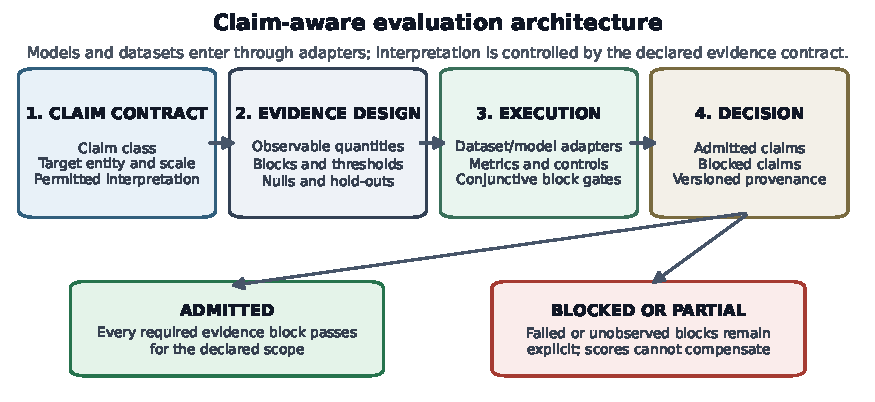
\includegraphics[width=0.72\linewidth]{figures/framework_workflow.pdf}
  \caption{MouseBrainBench workflow from claim declaration and
  observability analysis to evidence-block evaluation and the final claim gate.}
  \label{fig:framework-workflow}
\end{figure}

\subsection{Claim representation and evidence contract}
\label{subsec:claim-contract}

Let $\mathcal{M}$ denote a computational model, $\mathcal{D}$ an evaluation
dataset, and $C$ the scientific claim made about their relationship.
Conventional benchmarking estimates a predictive utility
$U(\mathcal{M},\mathcal{D})$ and ranks models using that scalar. This operation
is appropriate when $C$ is restricted to held-out prediction under a fixed
protocol. It is insufficient when the interpretation states that
$\mathcal{M}$ reproduces anatomical organization, identifies directed
dynamics, or represents a biological mechanism. Several models can provide
similar predictions while encoding incompatible structures or relying on a
common unobserved driver.

MouseBrainBench therefore represents an evaluation task as
\[
\mathcal{T}=\left(C,\mathcal{O},\mathcal{B},\mathcal{N},\mathcal{R},\mathcal{P}\right),
\]
where $\mathcal{O}$ contains the observable quantities, $\mathcal{B}$ is the
set of evidence blocks required by the claim, $\mathcal{N}$ defines the null
and alternative models, $\mathcal{R}$ contains the decision rules, and
$\mathcal{P}$ records provenance. A task is evaluable only when the quantities
needed by its evidence blocks are observable in $\mathcal{D}$. The framework
does not infer missing anatomical or interventional evidence from predictive
performance. An unevaluable block is reported as missing evidence and the
corresponding claim remains blocked.

Four claim classes are used in the present study. A \emph{predictive claim}
states that a model improves held-out neural-response prediction over declared
baselines. A \emph{reproducibility claim} states that an empirical target is
stable across repeated stimuli, partitions, sessions, or animals. A
\emph{structure--function claim} states that a structural relation remains
associated with a functional descriptor after relevant anatomical controls. A
\emph{mechanistic-identifiability claim} additionally requires the proposed
topology and direction to be distinguishable from plausible alternatives.
These classes form a partial order rather than a universal quality scale. A
useful predictor need not recover a circuit, while a reproducible local
structure--function association can remain weaker than intervention-supported
causality.

The scope of digital-twin terminology follows the same rule. An individual
whole-brain twin would require entity-specific calibration, sufficiently broad
structure and dynamics, repeated state estimation, and validation under
perturbations. None of the datasets used here jointly provides those
observations. Consequently, the current framework can audit partial digital
representations, but it cannot promote them to a complete or behavioural mouse
brain twin.

\subsection{Non-compensatory decision model}
\label{subsec:decision-model}

Each evidence block answers one validation question. The canonical mechanistic
configuration contains reproducibility, topology specificity, and directed
identifiability. Predictive evaluations add held-out performance, empirical
reliability, and out-of-distribution behaviour. Local structure--function
evaluations use matched anatomical controls, multiplicity correction, and
non-overlapping internal hold-out reproduction. Computational cost is recorded as an engineering
property but cannot substitute for biological evidence.

For criterion $j$ in block $i$, let $x_{ij}$ be the observed value, $t_{ij}$
its fixed threshold, and $d_{ij}$ the comparison direction. Criterion passage
is
\[
p_{ij}=\mathbb{I}\!\left[x_{ij}\ d_{ij}\ t_{ij}\right].
\]
For a criterion that requires a value larger than its threshold, the normalized
diagnostic score is
\[
s_{ij}=\min\!\left(1,\max\!\left(0,\frac{x_{ij}}{t_{ij}}\right)\right).
\]
The inverse ratio is used when smaller values provide stronger evidence, while
zero-threshold criteria receive one when they pass and zero otherwise. The
descriptive score of block $i$ is
\[
S_i=\frac{1}{n_i}\sum_{j=1}^{n_i}s_{ij},
\]
whereas block passage is $P_i=\bigwedge_j p_{ij}$. For $m$ required blocks,
the \ac{mis} and final decision are
\[
M=\frac{1}{m}\sum_{i=1}^{m}S_i,
\qquad
P_{\mathrm{MIS}}=\bigwedge_{i=1}^{m}P_i.
\]

The distinction between $M$ and $P_{\mathrm{MIS}}$ is central to the method.
The continuous value locates weak blocks and supports threshold-sensitivity
analysis, but it is not evidence that can be exchanged across blocks. A high
reproducibility score cannot compensate for a topology that performs like a
permuted graph. Similarly, a resolvable lead--lag signature cannot compensate
for failure to distinguish the proposed regional organization. The categorical
decision is therefore conjunctive, while the score remains diagnostic. This
prevents the numerical average from becoming an unsupported ranking of
mechanistic truth.

Null models are selected according to the claim. Permuted and disconnected
graphs test whether organization contributes beyond generic activity.
Transposed graphs test direction when the observable temporal resolution makes
that comparison meaningful. Mean-response, scrambled-stimulus, and transparent
temporal baselines test predictive value. Random, distance-matched, and
degree-matched non-connected pairs test local structure--function associations.
A null model is not considered adequate merely because it is computationally
convenient. It must remove the property under examination while preserving the
main nuisance structure that could otherwise explain the effect.

\subsection{Software architecture, construction, and execution workflow}
\label{subsec:software-workflow}

The implementation follows the six stages shown in
Fig.~\ref{fig:framework-workflow}. A configuration first declares the claim,
target scale, required evidence blocks, thresholds, and permitted conclusions.
Typed data schemas then describe regions, observations, predictions,
connectivity, subject identifiers, and provenance. Dataset adapters convert
Allen, Sensorium, Dynamic Sensorium, and \acs{microns} artifacts into those schemas
without erasing source-specific metadata. Model adapters expose outputs from
transparent baselines or external software through the same evaluation
interface. The validation layer computes metrics and null comparisons. The
claim gate evaluates each criterion and produces both a diagnostic report and a
bounded interpretation.

This separation was introduced incrementally. The first implementation
established common schemas, deterministic simulation runners, and basic
anatomical and predictive metrics. Known-truth systems were then added to test
the semantics of the decision rule before real data were admitted. Allen and
Sensorium adapters introduced repeated observations, subject-level partitions,
and predictive baselines. The \acs{microns} adapter added versioned \acs{cave} queries,
pair construction, anatomical matching, false-discovery-rate correction, and
unit-cluster bootstrap inference. At each stage, a component was retained only
when its output could be traced to a public resource or a deterministic
synthetic generator.

The resulting package separates data loaders, atlas and connectivity utilities,
dynamics, simulation, perturbations, validation metrics, baseline adapters,
visualization, and benchmark commands. This modularity is functional rather
than cosmetic. A new simulator can be connected through an adapter without
changing the definition of a claim. A new dataset can supply additional
observables without redefining how existing evidence blocks pass. A new
criterion can be introduced without altering archived outcomes. External tools
therefore remain responsible for simulation or prediction, while
MouseBrainBench controls evaluation semantics.

Each benchmark command writes a machine-readable artifact containing the
software revision, configuration, input identifiers, sample counts, random
seeds, thresholds, statistics, criterion directions, block decisions, and final
interpretation. A publication-freeze command reads those sealed artifacts and
emits two explicit lists: claims supported by the current evidence and claims
that remain blocked. It does not recalculate primary statistics or permit
manual replacement of headline values. This design makes the connection between
reported results and executable evidence auditable and prevents later narrative
changes from silently modifying the computational conclusion.

The same architecture also explains the role of each dataset. Synthetic systems
test decision logic under known truth. Allen provides a reproducible real-data
negative mechanistic control. Static and Dynamic Sensorium test whether modern
predictive gains remain separated from anatomical and causal claims. \acs{microns}
provides co-registered local structure and function for a bounded positive
association. These resources are complementary observations in one audit, not
interchangeable evidence for a single brain model.

\section{Experimental evaluation}
\label{sec:evaluation}

Several experiments have been carried out to evaluate the viability and
scientific usefulness of MouseBrainBench. The objective is not to rank
heterogeneous datasets or to claim that they jointly describe one complete mouse
brain. The objective is to test whether the framework can distinguish different
kinds of evidence and block interpretations that are not supported by the
available data.

The evaluation is organised around three research questions. \textbf{RQ1} asks
whether the non-compensatory decision rule recovers a known mechanism and
rejects reproducible but incomplete alternatives. \textbf{RQ2} asks whether the
framework preserves useful predictive evidence while preventing its promotion to
anatomical or causal interpretation. \textbf{RQ3} asks whether the same audit can
admit a positive structure--function result when the endpoint survives matched
controls and two non-overlapping internal hold-out windows. Table
\ref{tab:experimental-matrix} summarizes the resources, experimental units,
comparisons, and intended decisions.

\begin{table*}[t]
\centering
\caption{Experimental matrix used to evaluate the three research questions. The
resources are assigned different evidential roles and are not pooled as if they
were repeated measurements of one system.}
\label{tab:experimental-matrix}
\scriptsize
\begin{tabularx}{\textwidth}{@{}p{0.8cm}p{2.6cm}p{2.7cm}X X@{}}
\toprule
RQ & Resource and scale & Experimental units & Main comparisons & Decision target \\
\midrule
RQ1 & Four synthetic systems & 24 sessions, 6 regions per system & Directed truth, common drive, topology without direction, and direction without topology specificity & Recovery of known truth and rejection of incomplete mechanisms \\
RQ1 & Allen Visual Behavior Neuropixels & 20 sessions for reproducibility and topology, plus 21 sessions for direction & Cross-mouse and split-half stability, permuted and disconnected topology, latency and lead--lag nulls & Reproducible target without unsupported topology or direction \\
RQ2 & Static Sensorium & 7 validation mice and 5 repeated-test mice & Mean response, ridge predictors, scrambled stimulus, empirical reliability, and topographic null & Predictive and partial structural evidence kept separate from mechanism \\
RQ2 & Dynamic Sensorium & 5 current and 5 legacy out-of-distribution mice & Mean response, temporal filterbank, temporal SVD, random features, MLP, and bounded official-stack run & Paired predictive gain and software interoperability without leaderboard claims \\
RQ3 & MICRONS CAVE & 2991 units, 6575 synapses, 5943 unique connected directed pairs & Random, distance-matched, and degree-matched non-connected pairs, with discovery plus two hold-outs & Internally reproduced local observational structure--function association \\
\bottomrule
\end{tabularx}
\end{table*}


The exploratory and confirmatory status of the experiments is also fixed at this
point of the evaluation. The synthetic systems, Allen negative control, and
Sensorium analyses are framework-validation experiments: they test whether the
audit preserves prediction, reproducibility, topology, or direction only when the
corresponding evidence is observable. They are not pooled as biological evidence
for a single model. In the \acs{microns} experiment, the discovery window is used
for a narrower purpose. It diagnoses the failure of a broad aggregate
structure--function endpoint after distance matching and fixes the more specific
`all-pairs/readout-location' endpoint. The two subsequent windows are then used
as non-overlapping internal hold-outs. Therefore, discovery values are reported
for continuity and effect-size description, while the hold-out support for
the biological endpoint comes from the two non-overlapping hold-out windows and
the unit-cluster stability analysis. This design avoids presenting the stratified
search as if all positive subgroups were independent biological discoveries.

All thresholds, random seeds, cohort definitions, and criterion directions were
stored in benchmark configurations. Analyses were performed at the level of the
biological unit appropriate to each resource: session or mouse for population
recordings, and neuron-clustered resampling for connectomic pairs. Negative
results were retained because they test whether the framework blocks an
unsupported interpretation. The experiments therefore contain both passage and
failure by design.


\subsection{RQ1: known-truth recovery and the Allen negative control}
\label{subsec:rq1-known-truth-allen}

The first part of RQ1 uses four controlled systems containing 24 sessions, six
regions, and 24 temporal samples per session. Regional activity is generated
from Gaussian temporal profiles. A directed system introduces a latency shift
of 0.08 time units per region together with region-specific changes in amplitude
and width. Session noise has standard deviation 0.08, while independent
odd--even perturbations used for split-half evaluation have standard deviation
0.04. Fixed seeds 11, 23, 31, and 43 identify the directed-truth, common-drive,
topology-without-direction, and direction-without-topology systems.

Reproducibility is quantified by the median correlation between each session
and its system template, the median odd--even correlation, and the fraction of
sessions exceeding the 95th percentile of 200 within-session region
permutations. Topology specificity compares the candidate model with 100
region-permuted predictions and a disconnected template. Direction is evaluated
using resolvable peak latencies and nonzero lead--lag fractions. These systems
isolate complementary failure modes: common drive produces stable activity
without regional organization. Topology without direction contains structured
regional amplitudes with simultaneous peaks. Direction without topology
contains staggered peaks while the candidate does not outperform the
disconnected alternative. Only the directed-truth system is expected to pass
all blocks.

The observed decisions followed that expectation. The directed system passed
reproducibility, topology, and direction, obtaining $M=1.000$. The common-drive
system was highly reproducible but failed topology and direction
($M=0.333$). The topology-only system passed reproducibility and topology but
failed direction ($M=0.667$). The direction-only system contained temporal
information but failed topology specificity ($M=0.719$). In the directed case,
median cross-session and split-half correlations were 0.988 and 0.994. Candidate
prediction exceeded the median permuted prediction by 0.783 and the
disconnected prediction by 0.916. Every regional pair had resolvable
latency. By contrast, the common-drive system reached cross-session correlation
0.962 while its candidate prediction was 0.0009 worse than the permutation
median and 0.0032 worse than the disconnected control. These cases demonstrate
why the continuous \acs{mis} cannot replace the conjunctive decision: partial scores
locate a failure but do not constitute a ranking of mechanistic truth.

The second part of RQ1 examines whether the same rule remains conservative on a
real and strongly reproducible resource. Allen \ac{vbn}
artifacts were aggregated into regional population responses using fixed
windows and preprocessing. The reproducibility analysis contained 20 successful
sessions. The topology analysis used 20 sessions from 20 unique mice, and the
direction analysis used 21 sessions from 19 mice. The reproducibility block
required median cross-mouse correlation above 0.50, median split-half
correlation above 0.70, and at least half of sessions above their own
95th-percentile null. The topology block required the Allen-informed candidate
to improve by more than 0.05 over both the median permutation and a disconnected
model, outperform at least 95\% of permutations, and retain a positive paired
bootstrap lower bound. Direction required stable latency ordering, a sufficient
fraction of resolvable regional pairs, and lead--lag statistics above matched
nulls.

Allen produced the intended real negative control. Median cross-mouse
correlation was 0.891, median split-half correlation was 0.990, and 75\% of
sessions exceeded their own null. All reproducibility criteria passed. The
topological conclusion was the opposite. The Allen-informed candidate performed
0.0054 worse than the median permutation, outperformed only 21\% of
permutations, and improved by only 0.0035 over the disconnected model. None of
the topology criteria passed and the block score was 0.073. Median cross-mouse
and split-half latency agreement, the fraction above the latency null, the
resolvable-pair fraction, and the nonzero lead--lag fraction were all zero under
their operational definitions. The complete \acs{mis} was 0.358 and the decision was
\path{reproducible_target_without_mechanistic_identifiability}.

This outcome was stable when all Allen thresholds were multiplied by 0.75,
1.00, and 1.25. Reproducibility passed and both mechanistic blocks failed in
every condition. The experiment does not establish that the visual system lacks
directed organization. It establishes that the selected population target and
model comparison do not identify that organization. RQ1 is therefore answered
positively: the audit recovers complete synthetic truth, diagnoses incomplete
synthetic systems, and resists promoting highly reproducible real observations
to a mechanism.

\subsection{RQ2: predictive evidence in Static and Dynamic Sensorium}
\label{subsec:rq2-sensorium}

Static Sensorium was evaluated on seven validation mice and five mice with
repeated test stimuli. Neural responses were compared with a
stimulus-independent mean response, ridge regression over image features, and
ridge regression over image and behavioural covariates. A scrambled-stimulus
control preserved response distributions while breaking stimulus--response
assignment. Pearson correlation was computed on held-out observations and
summarized at mouse level. Repeated stimuli supplied an empirical reliability
estimate. Tiers without repetitions were not assigned an inferred reliability
value. A separate topographic analysis tested whether similarity in response
descriptors varied systematically with recorded spatial organization. Its
Spearman association and effect over a matched null were retained as partial
structural evidence, not interpreted as synaptic connectivity.

Across the seven validation mice, median best correlation was 0.328, median
improvement over mean response was 0.102, and median improvement over the
scrambled-stimulus control was 0.077. In the five repeated-test mice, median
reliability was 0.642 and median best predictive correlation was 0.341.
improvements over mean response and scrambled stimulus were 0.095 and 0.068.
The topographic constraint passed in all five datasets, with median Spearman
association 0.177 and median effect over its null 0.178. Reliability and
topographic evidence passed all six combinations obtained from reliability
thresholds 0.50 or 0.60 and topographic thresholds 0.05, 0.10, or 0.15. Passage
failed when the reliability threshold was raised to 0.70. This result is
informative but bounded: stimulus-aware models predict held-out responses and
partial topographic evidence is stable, while synaptic topology and causal
direction remain unobserved.

Dynamic Sensorium tested whether that distinction survives a more demanding
temporal task. Five current public mice and five legacy out-of-distribution mice
were evaluated with seven model families: mean response, summary features,
temporal filterbank, temporal \ac{svd}, random features, a compact PyTorch
\ac{mlp}, and a bounded model
instantiated through the official Sensorium loader and model factory. Models
were compared within mouse so that between-animal differences could not be
mistaken for architectural gains. The transparent temporal baselines provide a
meaningful intermediate comparison: the filterbank represents finite temporal
kernels, while temporal \acs{svd} estimates a low-rank temporal subspace. Random
features test whether nonlinear expansion alone explains an improvement, and
the \acs{mlp} tests a compact learned nonlinear mapping.

Best mouse-level correlations ranged from 0.427 to 0.526 in the current cohort.
The temporal filterbank won one mouse, temporal \acs{svd} won two, and the \acs{mlp} won
two. The filterbank improved over mean response in all five mice with median
gain 0.031. The \acs{mlp} median gain over mean response was 0.043, but its median
advantage over temporal \acs{svd} was only 0.0039. In the legacy out-of-distribution
cohort, the corresponding gains were 0.036 and 0.0022. At a required minimum
effect of 0.01, the \acs{mlp} surpassed temporal \acs{svd} in only one of five mice in each
cohort. Increased complexity therefore improved the simple baseline more
consistently than it improved a serious transparent temporal model.

The bounded official-architecture run completed through the official Sensorium
loader and model factory for five mice, with correlations from 0.011 to 0.035
under a deliberately restricted training budget. These values are neither
evidence against the official architecture nor a competitive baseline. Their
role is to verify that data loading, model construction, training, and
evaluation execute within the MouseBrainBench environment. The audit marks this
artifact as an interoperability control and blocks state-of-the-art or
leaderboard-equivalent interpretations because the published training budget
and protocol were not reproduced.

RQ2 is also answered positively, although not by obtaining a new leading
predictor. MouseBrainBench preserves prediction, repeat reliability,
out-of-distribution behaviour, and topographic association as separate outcomes.
It identifies when a neural model improves a transparent baseline and when that
gain becomes marginal after a stronger temporal comparison. None of these
results is allowed to satisfy the missing synaptic or interventional evidence.

The robustness and ablation analyses in Fig.~\ref{fig:sensitivity-ablation}
examine whether these decisions depend on a single favourable threshold or on a
weak comparator. For Allen, multiplying every criterion threshold by 0.75,
1.00, or 1.25 leaves the block pattern unchanged: reproducibility passes while
topology and direction fail. For Static Sensorium, the topographic criterion
passes throughout the tested range, whereas the combined partial-positive gate
fails when required reliability rises from 0.60 to 0.70. The boundary is thus
attributable to empirical response reliability rather than to re-selection of
the topographic effect.

\begin{figure}[pos=tp]
  \centering
  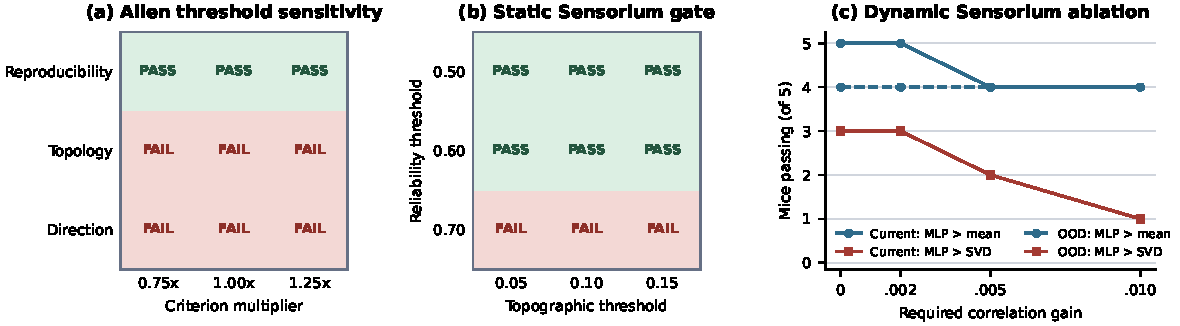
\includegraphics[width=0.88\linewidth]{figures/sensitivity_ablation.pdf}
  \caption{Sensitivity and ablation results for Allen, Static
  Sensorium, and Dynamic Sensorium. Solid lines denote the current cohort and
  dashed lines the legacy out-of-distribution cohort.}
  \label{fig:sensitivity-ablation}
\end{figure}

The Dynamic Sensorium panel provides an ablation over comparator strength and
minimum effect. At zero or 0.002 required gain, the \acs{mlp} exceeds temporal \acs{svd} in
three of five mice in each cohort. At 0.005 this falls to two mice, and at 0.010
to one. By contrast, gains over mean response remain in four or five mice over
the same range. The apparent neural-network advantage is therefore robust to a
weak baseline but not to a stronger temporal decomposition. This result is not
used to reject the \acs{mlp}. It establishes the narrower conclusion that model
complexity alone is not the source of the predictive evidence and that claims
of architectural superiority depend materially on the comparator and minimum
effect selected.

\subsection{RQ3: MICRONS structure--function validation and cross-regime synthesis}
\label{subsec:rq3-microns}

\acs{microns} supplies the local co-registration required for a positive
structure--function test. Data were queried from the public
\path{minnie65_public} \ac{cave} stack. Functional descriptors were obtained from
\path{digital_twin_properties_bcm_coreg_v4}, structural edges were
queried at materialization version 1507, and acquisition artifacts recorded the
datastack, table, materialization, offsets, limits, and source identifiers.
Three non-overlapping ordered windows defined discovery and internal
hold-out reproduction. Offset 0 provided 1000 usable units, offset 1000 provided
992, and offset 2000 provided 999. Structural queries yielded 2267, 2161, and
2147 synapses, corresponding to 2095, 1926, and 1922 unique connected directed
pairs. The windows were evaluated separately rather than pooled before
validation. They are internal windows from the same MICRONS resource and should
not be interpreted as independent-animal replication.

An initial discovery analysis compared connected pairs with random,
distance-matched, and degree-matched non-connected pairs across multiple
functional descriptors. Connected pairs were more similar than random and
degree-matched controls, but the aggregate contrast did not survive distance
matching. Since cortical distance affects both connection probability and
functional organization, this failure blocked the broad positive conclusion.
The diagnostic result was retained and readout-location similarity was selected
as a narrower endpoint before the hold-out windows were evaluated. This sequence
is important: the random control alone would have produced an overstated result,
whereas the distance-matched gate forced a bounded claim that could be
evaluated in predeclared non-overlapping hold-out windows.

For each connected directed pair, random non-connected pairs estimated the
unconditioned contrast, distance-matched pairs controlled for spatial
separation, and degree-matched pairs controlled for unequal participation of
high-degree neurons. The effect $\Delta$ was defined as connected-pair
similarity minus control-pair similarity. One-sided tests evaluated the
declared positive direction, and the Benjamini--Hochberg procedure controlled
the false discovery rate within each stratified family. Because one neuron can
contribute to many pairs, uncertainty was estimated with 300 unit-cluster
bootstrap samples using seed 71. Resampling units induces weights over the existing directed pair frame and
avoids the false precision obtained when derived pairwise observations are
treated as independent.

The three cohorts jointly contained 2991 units, 6575 loaded synapses, and 5943
unique connected directed pairs. Table~\ref{tab:microns-primary} reports the
primary matched effects. The values $\Delta_d$ and $\Delta_k$ denote the
difference between the mean readout-location similarity of connected directed
pairs and the corresponding non-connected null matched by distance or degree.
Positive values indicate that connected pairs are more similar under the
reported functional descriptor. Readout-location similarity is a derived
functional descriptor from the MICrONS digital-twin table and is normalized as
a similarity score for comparison; it is not a direct causal measurement of
synaptic influence. Distance-matched effects were 0.0215, 0.0210, and 0.0179
in discovery, hold-out 1000, and hold-out 2000, with adjusted $q$ values of
0.0076, 0.0070, and 0.0087. Degree-matched effects were 0.0403, 0.0380, and
0.0286, with adjusted $q$ values of 0.0053, 0.0062, and 0.0083. The effect
therefore retained its sign and approximate magnitude outside the window used
to establish the endpoint.

\begin{table}[t]
\centering
\caption{Internally reproduced MICRONS primary endpoint. $\Delta_d$ and $\Delta_k$ are differences between connected-pair readout-location similarity and non-connected nulls matched by distance or degree; positive values indicate greater similarity among connected pairs. The readout-location descriptor is derived and must not be interpreted as causal evidence.}
\label{tab:microns-primary}
\small
\begin{tabular}{lrrrrrr}
\toprule
Cohort & Units & Connected & $\Delta_d$ & $q_d$ & $\Delta_k$ & $q_k$ \\
\midrule
Discovery & 1000 & 2095 & 0.0215 & 0.0076 & 0.0403 & 0.0053 \\
Hold-out 1000 & 992 & 1926 & 0.0210 & 0.0070 & 0.0380 & 0.0062 \\
Hold-out 2000 & 999 & 1922 & 0.0179 & 0.0087 & 0.0286 & 0.0083 \\
\bottomrule
\end{tabular}
\end{table}

Unit-cluster bootstrap stability intervals remained strictly positive in every
cohort (Table~\ref{tab:microns-bootstrap}). Distance-matched lower bounds were
0.0166, 0.0142, and 0.0115. Degree-matched lower bounds were 0.0349, 0.0321,
and 0.0229. All 300 requested bootstrap samples were usable. Because directed
pairs share neurons, these intervals are reported as a unit-cluster stability
analysis and are not treated as if pairwise observations were independent. The
discovery family contained 174 tests across descriptors and strata, of which
28 were confirmed after false-discovery-rate correction. The hold-outs
contained 162 and 174 tests, with 30 and 25 confirmed positives. These counts
describe the multiplicity families and are not presented as independent
biological discoveries. The main claim rests on the fixed readout-location
endpoint and its internal reproduction.

\begin{table}[t]
\centering
\caption{Unit-cluster bootstrap stability analysis for the MICRONS primary endpoint using 300 resamples per cohort. PI denotes a 95\% percentile interval. Intervals are reported as robustness summaries for neuron-sharing pair data, not as naive pair-level uncertainty estimates.}
\label{tab:microns-bootstrap}
\small
\begin{tabular}{lrrrr}
\toprule
Cohort & Distance median & Distance 95\% PI & Degree median & Degree 95\% PI \\
\midrule
Discovery & 0.0218 & [0.0166, 0.0263] & 0.0405 & [0.0349, 0.0454] \\
Hold-out 1000 & 0.0209 & [0.0142, 0.0263] & 0.0377 & [0.0321, 0.0431] \\
Hold-out 2000 & 0.0181 & [0.0115, 0.0238] & 0.0287 & [0.0229, 0.0354] \\
\bottomrule
\end{tabular}
\end{table}

The \acs{microns} outcome is an internally reproduced local observational association, not a new
wiring rule or a causal mechanism. Readout-location similarity may still covary
with cell type, layer, cortical area, morphology, or developmental organization.
Distance and degree matching address two major confounds but do not exhaust the
causal graph. Moreover, Ding et al. reported a substantially richer analysis of
like-to-like connectivity using receptive fields, feature preference, and
axon--dendrite geometry \citep{ding2025wiring}. The present result serves as a
connectomic validation case for the audit: it shows that MouseBrainBench can admit a
positive, internally reproduced claim without asserting priority over the
underlying biological phenomenon.

Table~\ref{tab:cross-regime-results} brings the complete evaluation together.
The important outcome is not that one resource attains the highest score. The
same executable logic represents complete synthetic passage, incomplete
mechanistic systems, reproducible but non-identifying Allen activity,
predictive Sensorium models, and a local positive \acs{microns} association without
semantic promotion. Compared with a conventional evaluation that mainly reports
prediction or reproducibility, this non-compensatory gate prevents Allen and
Sensorium results from being promoted to mechanistic conclusions and restricts
MICRONS to an internal local association. The publication freeze consequently admits those bounded
interpretations while blocking a complete mouse-brain digital twin,
state-of-the-art Sensorium prediction, causal identifiability, behavioural
claims, and whole-brain extrapolation.

\begin{table*}[t]
\centering
\caption{Cross-regime outcomes produced by the same claim-aware audit. Positive
evidence is retained without promoting it to a stronger interpretation.}
\label{tab:cross-regime-results}
\scriptsize
\begin{tabularx}{\textwidth}{@{}p{2.4cm}p{3.3cm}p{3.3cm}X@{}}
\toprule
Case & Positive evidence & Failed or unavailable evidence & Admissible interpretation \\
\midrule
Synthetic directed truth & All reproducibility, topology, and direction blocks pass with $M=1.000$ & None under the designed mechanism & Complete recovery of the synthetic mechanism \\
Synthetic incomplete cases & Strong partial scores ($M=0.333$--$0.719$) & At least one required topology or direction block fails & Diagnostic partial evidence with mechanistic passage rejected \\
Allen VBN & Cross-mouse correlation 0.891 and split-half correlation 0.990 & Topology block 0.073, failed direction criteria, and complete MIS 0.358 & Reproducible population target without identified organization \\
Static Sensorium & Median best correlation 0.328, repeated-test reliability 0.642, and topographic association 0.177 & Reliability unavailable for non-repeated tiers, with no synaptic graph or causal direction & Predictive utility with partial reliability and topographic evidence \\
Dynamic Sensorium & Best mouse-level correlations 0.427--0.526 and MLP median gain 0.043 over mean response & Small gain over temporal SVD (0.0039), while the bounded official run is not competitive & Temporal predictive evidence and verified software integration \\
MICRONS & Distance-matched effects 0.0215, 0.0210, 0.0179 and positive clustered stability intervals in all cohorts & No intervention, same animal/resource, with residual cell-type, layer, area, and morphology confounding & Internally reproduced local observational structure--function association \\
\bottomrule
\end{tabularx}
\end{table*}

\section{Discussion}
\label{sec:discussion}

The results show that MouseBrainBench addresses a narrow but relevant problem in
computational neuroscience. Current models can predict neural measurements with
increasing accuracy, but the language used to describe them can easily move from
prediction to mechanism or digital-twin fidelity. The proposed framework makes
this transition explicit and testable. Synthetic systems reveal which evidence
block is absent, Allen keeps a reproducible target while rejecting topology and
direction, Sensorium keeps predictive usefulness without causal interpretation,
and \acs{microns} admits a bounded local structure--function association after
matched controls and hold-out confirmation.

\subsection{Comparison with existing benchmark and validation paradigms}
\label{subsec:benchmark-comparison}

MouseBrainBench differs from predictive neuroscience benchmarks primarily in
its unit of evaluation. Sensorium evaluates a model on a defined prediction
task and provides a common basis for comparing architectures. That design is
appropriate for determining which predictor generalizes better under the
competition protocol \citep{willeke2022sensorium,turishcheva2023dynamic}.
MouseBrainBench instead evaluates the relationship between an empirical result
and the interpretation attached to it. Predictive correlation is retained as
one observation, but the benchmark instance also records whether repeated
responses are reliable, whether a proposed topology outperforms plausible
alternatives, and whether directional or interventional information is
observable. Consequently, the framework does not replace a leaderboard. It
determines which conclusions may legitimately be exported from one.

The distinction from simulation infrastructures is equally important. \acs{bmtk},
SONATA-compatible workflows, \acs{tvb}, and The Virtual Mouse Brain
provide mature mechanisms for constructing networks, executing dynamics, and
exchanging model descriptions \citep{dai2020bmtk,tvb2013,melozzi2017virtualmouse}.
Their central engineering object is an executable model. The central object in
MouseBrainBench is an evidence contract. A simulator can therefore be connected
as a candidate model without reproducing its numerical engine, but successful
execution is not itself treated as biological validation. Model outputs must
still be compared with observables, controls, and independent data appropriate
to the proposed claim.

This position is consistent with the broader verification, validation, and
uncertainty-quantification literature, which treats model credibility as
purpose-dependent rather than absolute
\citep{asme2018vv40,oberkampf2010verification,sargent2013verification,riedmaier2021vvuq}.
Digital-twin credibility frameworks similarly emphasize intended use,
lifecycle evidence, data provenance, and uncertainty rather than assuming
that the twin label guarantees fidelity
\citep{jones2020digitaltwin,rasheed2020digitaltwin,fuller2020digitaltwin,shao2022credibility}. MouseBrainBench contributes a
domain-specific operationalization for AI-based neural models: it maps purpose
to required evidence blocks, makes those blocks non-interchangeable, and binds
the reported interpretation to sealed computational artifacts. It does not yet
provide a complete uncertainty-quantification treatment of parameters and
model form. Instead, threshold sensitivity, matched nulls, clustered intervals,
and hold-out reproduction cover the uncertainties directly estimable from the
present resources.

Four practical properties therefore delimit the methodological contribution.
First, the benchmark compares claims rather than forcing heterogeneous models
onto one scalar leaderboard. Second, evidence types retain their semantics:
prediction, reproducibility, topology, direction, and structure--function
association cannot compensate for one another. Third, failed criteria remain
publishable outputs, making negative controls part of validation rather than
discarded development information. Fourth, the publication freeze joins
software revision, data identifiers, thresholds, and admissible language. No
single property is unprecedented in isolation. The contribution lies in their
executable combination across predictive, simulation, and connectomic regimes.

The negative Allen result is scientifically useful. A less restrictive
benchmark might report cross-mouse correlation of 0.891 and split-half
correlation of 0.990 as validation of a model. MouseBrainBench instead asks
whether the Allen-informed topology performs better than alternatives and
whether a directed signature can be recovered. It does not. This outcome does
not contradict the biological organization of the visual system. It identifies
an observational limitation: repeatable population dynamics do not uniquely
determine the graph that generated them.

Sensorium illustrates a related distinction in modern \acs{ai}.
Static stimulus and context models improve prediction over mean and scrambled
controls, while temporal models and a compact neural network improve predictions
for Dynamic Sensorium. These are valid functional results. They are not evidence
that the architecture's internal variables correspond to synapses, cell types,
or causal operations in the animal. Treating predictive and mechanistic scores
as separate outputs allows the same model to be accepted for one purpose and
rejected for another without contradiction.

The bounded official Sensorium experiment also clarifies what software
integration demonstrates. Executing an official loader and architecture verifies
interoperability, but a restricted local training budget is not comparable with
a published competition result. The very low bounded correlations are therefore
neither evidence against the official architecture nor a competitive baseline.
They document that the integration path works and that a full-budget comparison
remains absent. This prevents an engineering smoke test from becoming an
inflated empirical claim.

The \acs{microns} result is the main positive empirical case, but its novelty must be
stated precisely. Ding et al. already demonstrated like-to-like connectivity
with a more extensive biological analysis, including feature, receptive-field,
and axon--dendrite geometry controls. MouseBrainBench does not improve that
biological finding. Instead, the \acs{microns} experiment tests whether a compact,
declared audit can recover a compatible local association and preserve its
proper scope. Internal reproduction across two non-overlapping windows and positive
unit-cluster bootstrap stability intervals provide a robustness check for the audit
pipeline.

The effect is not causal. Readout-location similarity can covary with cortical
area, layer, cell class, developmental organization, or unmeasured morphology.
Distance and degree matching address two major confounds but do not exhaust the
causal graph. In particular, the analysis does not compare axon--dendrite
opportunity at the resolution used by Ding et al., manipulate individual
connections, or demonstrate that the observed edges are necessary for the
functional descriptor. The permitted interpretation is therefore an internally reproduced
local observational association.

\subsection{Threats to validity and transfer beyond the mouse brain}
\label{subsec:validity-transfer}

The first threat concerns construct validity. \acs{mis} operationalizes mechanistic
identifiability through evidence blocks selected for the claim, but these blocks
are not a universal definition of mechanism. Latency and lead--lag information
are meaningful for the regional temporal systems examined here, whereas a
molecular pathway, a biophysical cell model, or a behavioural controller would
require different observables and alternatives. A passing decision means that
the declared operational criteria have been satisfied. It does not establish
that every scientifically plausible mechanism has been excluded. This is why
the continuous \acs{mis} value is diagnostic and why the categorical interpretation
must always be read together with the contract.

Internal validity is limited by the controls that can be constructed from each
resource. Permutations and disconnected models remove selected organizational
properties but cannot represent every latent circuit compatible with Allen
population activity. In \acs{microns}, distance and degree matching substantially
improve on random-pair comparison, yet cell class, laminar position, cortical
area, morphology, developmental lineage, and axon--dendrite opportunity may
still confound functional similarity. The aggregate analysis demonstrates the
importance of this issue: a positive random-pair contrast disappeared after
distance matching. The narrower internally reproduced endpoint reduces the overclaim but
does not turn an observational association into a causal effect.

Statistical conclusion validity is constrained by the number and independence
of biological units. Pairwise \acs{microns} observations share neurons and form
dyadic dependencies, so the study uses a unit-cluster weighted bootstrap rather
than naive pair resampling. This choice avoids treating all directed pairs as
independent observations, but it remains a practical robustness analysis rather
than a complete dyadic-inference treatment. In addition, the three cohorts are
disjoint windows from one animal, not independent biological replicates. Dynamic
Sensorium comparisons contain five mice per cohort. Win counts and medians are
consequently more informative than asymptotic claims. The sensitivity analysis
reduces dependence on one threshold, but its tested grid is finite and does not
replace external preregistration. Multiple descriptor and stratum tests are
false-discovery-rate corrected, while the main claim is restricted to the fixed
endpoint internally reproduced in both hold-outs. Future releases should
increase bootstrap samples and compare the current stability analysis against
robust methods for dyadic or network-dependent data.

External validity is bounded by species, brain area, task, and measurement
modality. Allen and Sensorium emphasize the mouse visual system. \acs{microns} covers
a restricted visual-cortical volume from one mouse, and the Allen experiments
use controlled subsets of the available sessions. The framework has not been
validated on subcortical circuits, longitudinal disease trajectories, freely
moving behaviour, closed-loop perturbation, or individual calibration across
modalities. These omissions directly block whole-brain and individual-twin
claims. They also mean that the current thresholds should not be transferred
unchanged to a different species or recording technology.

What can transfer is the evaluation grammar. A domain outside mouse neuroscience
can define a target claim, list the quantities that make it observable, specify
non-compensatory evidence blocks, construct claim-relevant alternatives, and
seal the resulting decision with provenance. In human neuroimaging, for
example, subject-level calibration and test--retest reliability might replace
session-level criteria, while interventions may remain unavailable. In
manufacturing, sensor calibration, operating-envelope coverage, and uncertainty
propagation would become mandatory blocks. In climate or physiological models,
conservation laws and out-of-regime validation could replace synaptic topology.
The software interfaces can represent these contracts, but scientific validity
still requires domain experts to justify the observables, controls, thresholds,
and consequences of failure.


The synthetic validation should also be interpreted with the appropriate scope. The four systems confirm that the implemented gate behaves as intended under controlled mechanisms, but they do not estimate operating characteristics over a broad generative family. They therefore do not yet provide false-positive or false-negative rates, threshold calibration curves, or robustness surfaces over noise, sample size, and gradual mechanism strength. A larger Monte Carlo benchmark is required before the MIS can be presented as a calibrated statistical test rather than as an executable claim-control rule.

The current \acs{mis} should also not be treated as a universal scalar definition of
mechanistic explanation. Its principal contribution is structural: evidence
blocks are non-interchangeable and passage criteria are explicit. The particular
criteria and thresholds remain claim-dependent. A molecular mechanism, a
neural-mass model, and an individual-level behavioural twin would require
different blocks. External preregistration and application by independent groups
are needed before \acs{mis} can be regarded as a community standard.

Conjunctive rules have an intentional cost. They reduce false promotion of
partial evidence but can reject scientifically interesting models when one
required measurement is unavailable. MouseBrainBench handles this by retaining
block scores and partial-positive labels. Failure of the global decision means
that the target claim is unsupported under the declared evidence. It does not
mean that the model, data, or partial result is useless. This semantic discipline
is important if the framework is to encourage stronger experiments rather than
merely produce negative labels.

The sensitivity analysis indicates that the main qualitative conclusions are
not artifacts of one exact threshold. Allen remains negative under 25\%
relaxation and tightening. Static Sensorium retains partial reliability and
topographic evidence for six of nine threshold combinations, failing when the
reliability threshold reaches 0.70. Dynamic Sensorium gains over mean response
are more stable than gains over temporal \acs{svd}, supporting predictive utility but
not superiority of a specific neural architecture. These patterns make the
limitations visible instead of hiding them in a single aggregate score.

For an engineering contribution in \acs{ai}, the value of the
work depends on the framework being useful beyond this exact collection of
analyses. The software interfaces are therefore organized around claims,
evidence blocks, graphs, predictions, perturbations, and provenance rather than
around hard-coded dataset names. External \acs{bmtk}, SONATA, or \acs{tvb}
simulations can be added as candidate models without reimplementing their
numerical engines. New datasets can add evidence blocks while retaining the
same publication-freeze contract.

The next scientific step is not to increase model complexity indiscriminately.
It is to add evidence unavailable here: independent-animal structure--function
replication, perturbations that distinguish competing mechanisms, and
full-budget predictive baselines. Those additions would test whether the audit
can move from observational association towards intervention-supported
mechanism. Until then, MouseBrainBench should be understood as a reproducible
claim-control framework for partial mouse-brain models, not as the mouse-brain
model itself.

\section{Conclusions}
\label{sec:conclusions}

This paper presented MouseBrainBench, a claim-aware verification and validation
framework for \acs{ai} models used as partial digital representations of the
mouse brain. The proposal tackles a relevant problem: predictive performance,
reproducibility, structural fidelity, and mechanistic identifiability are often
measured separately but interpreted as if they were interchangeable. To avoid
this situation, MouseBrainBench organises validation through explicit evidence
blocks, matched controls, and non-compensatory claim gates.

The Mechanistic Identifiability Score provides a diagnostic summary of the
available evidence. However, the final claim is not decided by a weighted
average. A claim passes only when all the required evidence blocks pass. The
synthetic experiments confirm this behaviour by rejecting common drive, topology
without direction, and direction without topology-specific prediction, even when
some partial evidence is strong. This fact is the main methodological
contribution of the work, as it turns validation assumptions into executable and
falsifiable contracts.

The real-data experiments produced complementary outcomes. Allen Visual Behavior
Neuropixels showed strong reproducibility, but did not identify the proposed
topology or direction. Static and Dynamic Sensorium provided predictive gains,
but the evidence was not sufficient to support a mechanistic or causal claim.
MICRONS provided the main positive empirical case: across a discovery cohort and two
non-overlapping hold-out windows from the same resource, connected directed
pairs showed greater readout-location similarity than distance- and
degree-matched controls, with positive unit-cluster bootstrap stability intervals.

It can be concluded that MouseBrainBench is useful as a claim-audit framework
for partial mouse-brain digital models. The current evidence supports a bounded
local observational structure--function claim in MICRONS and demonstrates that
several tempting broader claims must remain blocked. In particular, the paper
does not validate a complete mouse-brain digital twin, a causal mechanism, a
behavioural twin, or a state-of-the-art Sensorium predictor.

Future work should apply the framework to external simulators, including
biophysically detailed models, neural-mass models, and emerging digital-brain
proposals. It is also necessary to extend the framework towards intervention
experiments, broader subject-level replication, stronger uncertainty
quantification, larger Monte Carlo operating-characteristic studies, and direct
comparisons with conventional predictive-only evaluation. These extensions should preserve the central principle of the
proposal: every model output must be interpreted only according to the evidence
that has actually passed the declared claim gate.

\section{Data, code, and ethics statement}
\label{sec:data-code-availability}
This study performs a secondary analysis of public datasets. Therefore, it does
not introduce new animal experiments. Ethical approvals, animal-care procedures, and primary
data-acquisition protocols correspond to the original Allen, Sensorium, and
MICRONS studies. Raw public datasets are not redistributed.

Source code, configurations, acquisition scripts, and result artifacts are
available in an anonymous review archive. The public repository and archival DOI
will be disclosed after double-anonymized review. The archival package should
include the exact source revision, configuration files, result artifacts, figure
and table generation scripts, random seeds, software environment specification,
and the public identifiers or materialization versions used to acquire each
external resource. It should also retain the MICRONS stopping rule and volume
adequacy statement so that additional data cannot be used to redefine the
primary endpoint after manuscript preparation. Artifacts generated from a dirty
working tree should be regenerated from a clean commit before release. This
reproducibility manifest follows FAIR data, FAIR
software, and reusable-model guidance \citep{wilkinson2016fair,barker2022fair4rs,patel2023fairbiors,sauro2026cure}.
Data acquisition commands preserve public source identifiers and application
programming interface queries where licenses permit. MICRONS CAVE access
requires a personal token and acceptance of the service terms.


\section{Declaration of generative AI and AI-assisted technologies in the writing process}
\label{sec:generative-ai-declaration}
During the preparation of this work, the author used ChatGPT and OpenAI Codex to support language revision, code review, and manuscript structuring. The author reviewed and edited all generated material and takes full responsibility for the content of the publication.

\section{Declaration of competing interest}
\label{sec:competing-interest}
The author declares no known competing financial interests or personal
relationships that could have appeared to influence the work reported in this
paper.

\section{Acknowledgements}
\label{sec:acknowledgements}
This work has been funded by the Spanish MICIU under the PDI program in the
XMIDAS project (PID2021-122640OB-I00).

\printcredits
\bibliographystyle{cas-model2-names}
\bibliography{references}


\end{document}
